\chapter{Анализ результатов\label{chapter_2}}
\section{Особенности реализации}

При реализации методов, описанных в предыдущем пункте использовался язык C++, стандарт 2011 года.
Структура проекта была разбита на несколько составных частей:
\begin{itemize}
\item[1.] Описание численного метода Симпсона.
\item[2.] Описание численного метода Гаусса.
\item[3.] Описание граничных условий.
\item[4.] Описание самого процесса деформирования.
\end{itemize}

В первых двух пунктах был применена технология шаблонов, так как к функциям интегрирования обращаются объекты разных классов.
Шаблон(template)~--- средство языка C++, предназначенное для кодирования обобщённых алгоритмов, без привязки к некоторым параметрам (например, типам данных, размерам буферов, значениям по умолчанию). В C++ возможно создание шаблонов функций и классов.

В частности были написаны обобщенные функции интегрирования методом Гаусса и методом Симпсона, которые на вход принимали объект, у которого присутствовал оператор, вычисляющий значение подынтегральной функции, а тип объекта определен не был, так в эти функции передавались объекты различных классов. 

В стандарте C++11 появилась встроенная поддержка многопоточности, что также было использовано в работе.
Потоком в программировании называют легковесный процесс, имеющий с процессом-родителем общие ресурсы, такие как память, тогда как процессы не разделяют этих ресурсов. В частности, потоки разделяют инструкции процесса (его код) и его контекст (значения переменных, которые они имеют в любой момент времени).

Задача о деформировании мембраны внутри криволинейной матрицы связана с большим количеством вычислений интегралов. Алгоритм вычисления интеграла с неопределенным верхним пределом выглядит так:
\begin{itemize}
\item разбиваем область верхнего предела на отдельные участки;
\item вычисляем по каждому участку значение;
\item суммируем полученный результат, получая непрерывные значения.
\end{itemize}
		\begin{figure}[h!]
				\center{\includegraphics[width=0.7\linewidth]{images/img4.jpg}}
				\caption{ Время работы программы } 
				\label{parall_results}
	    \end{figure}

Как видно из алгоритма, второй пункт можно вычислять независимо для каждого интеграла. В результате разбиения задач по потокам для свободного и стесненного деформирования внутри криволинейной матрицы было получено ускорение отображаемое на рис.\ref{parall_results}. Отметим, что во второй задаче, где фигурирует матрица с вертикальными стенками и плоским днищем, результаты распараллеливания не приведены, так как там слишком малое время вычисления из-за упрощенных формул для вычисления толщины мембраны на каждом шаге, в силу вида матрицы.


	    
\section{Результаты\label{section_2}}
	В качестве примера рассмотрим деформирование мембраны из алюминиевого сплава Д16T при $400^\circ\text{C}$ [\ref{teraud}]. Константы материала: 
   $C=9.37\cdot10^5 \text{МПа}^{-n}\text{сек}^{-1}$, $n=3.4$, $\sigma_b = 88.3\; \text{МПа}$. 
   Геометрические размеры мембраны: ширина $2a=200$ мм, толщина $H_0=2$ мм, $k$=1.5, $\overline{b}$=4.5 давление $q=2.65$ кПа [\ref{teraud}].  
   
   Вычисления показали, что мембрана в условиях идеального скольжения полностью заполняет криволинейную матрицу $y=4.5(1-x^{1.5})$ за бесконечное время. 
   Стадия мгновенного деформирования характеризуется параметром $\overline{H}_1 = 0.97$, 
   стадия свободного деформирования характеризуется параметрами $\overline{H}_2 = 0.69, \overline{t}_2 = 5.36 \cdot 10^8$.
   На рис.\ref{quad_sliging} представлен график зависимости толщины мембраны и интенсивности напряжения от времени
   (кривые 1 и 2 соответственно).
   
   		\begin{figure}[h!]	
				\def\svgwidth{\columnwidth}
				\center{\includegraphics[width=0.9\linewidth]{images/quad_sliding.png}}
				\caption{} 
				\label{quad_sliging}
		\end{figure}

Расчет для прилипания, как граничного условия,	показал, что для начальных данных, идентичных случаю скольжения 
	мембрана разрушается при толщине $\overline{H}=0.015$ за время $\overline{t}=12.15\cdot 10^8$, достигая предельно доупстимого напряжения $\sigma_b$.    На рис.\ref{quad_sticking} представлен график зависимости толщины мембраны и интенсивности напряжения от времени (кривые 1 и 2 соответственно).
   
		\begin{figure}[h!]	
				\def\svgwidth{\columnwidth}
				\center{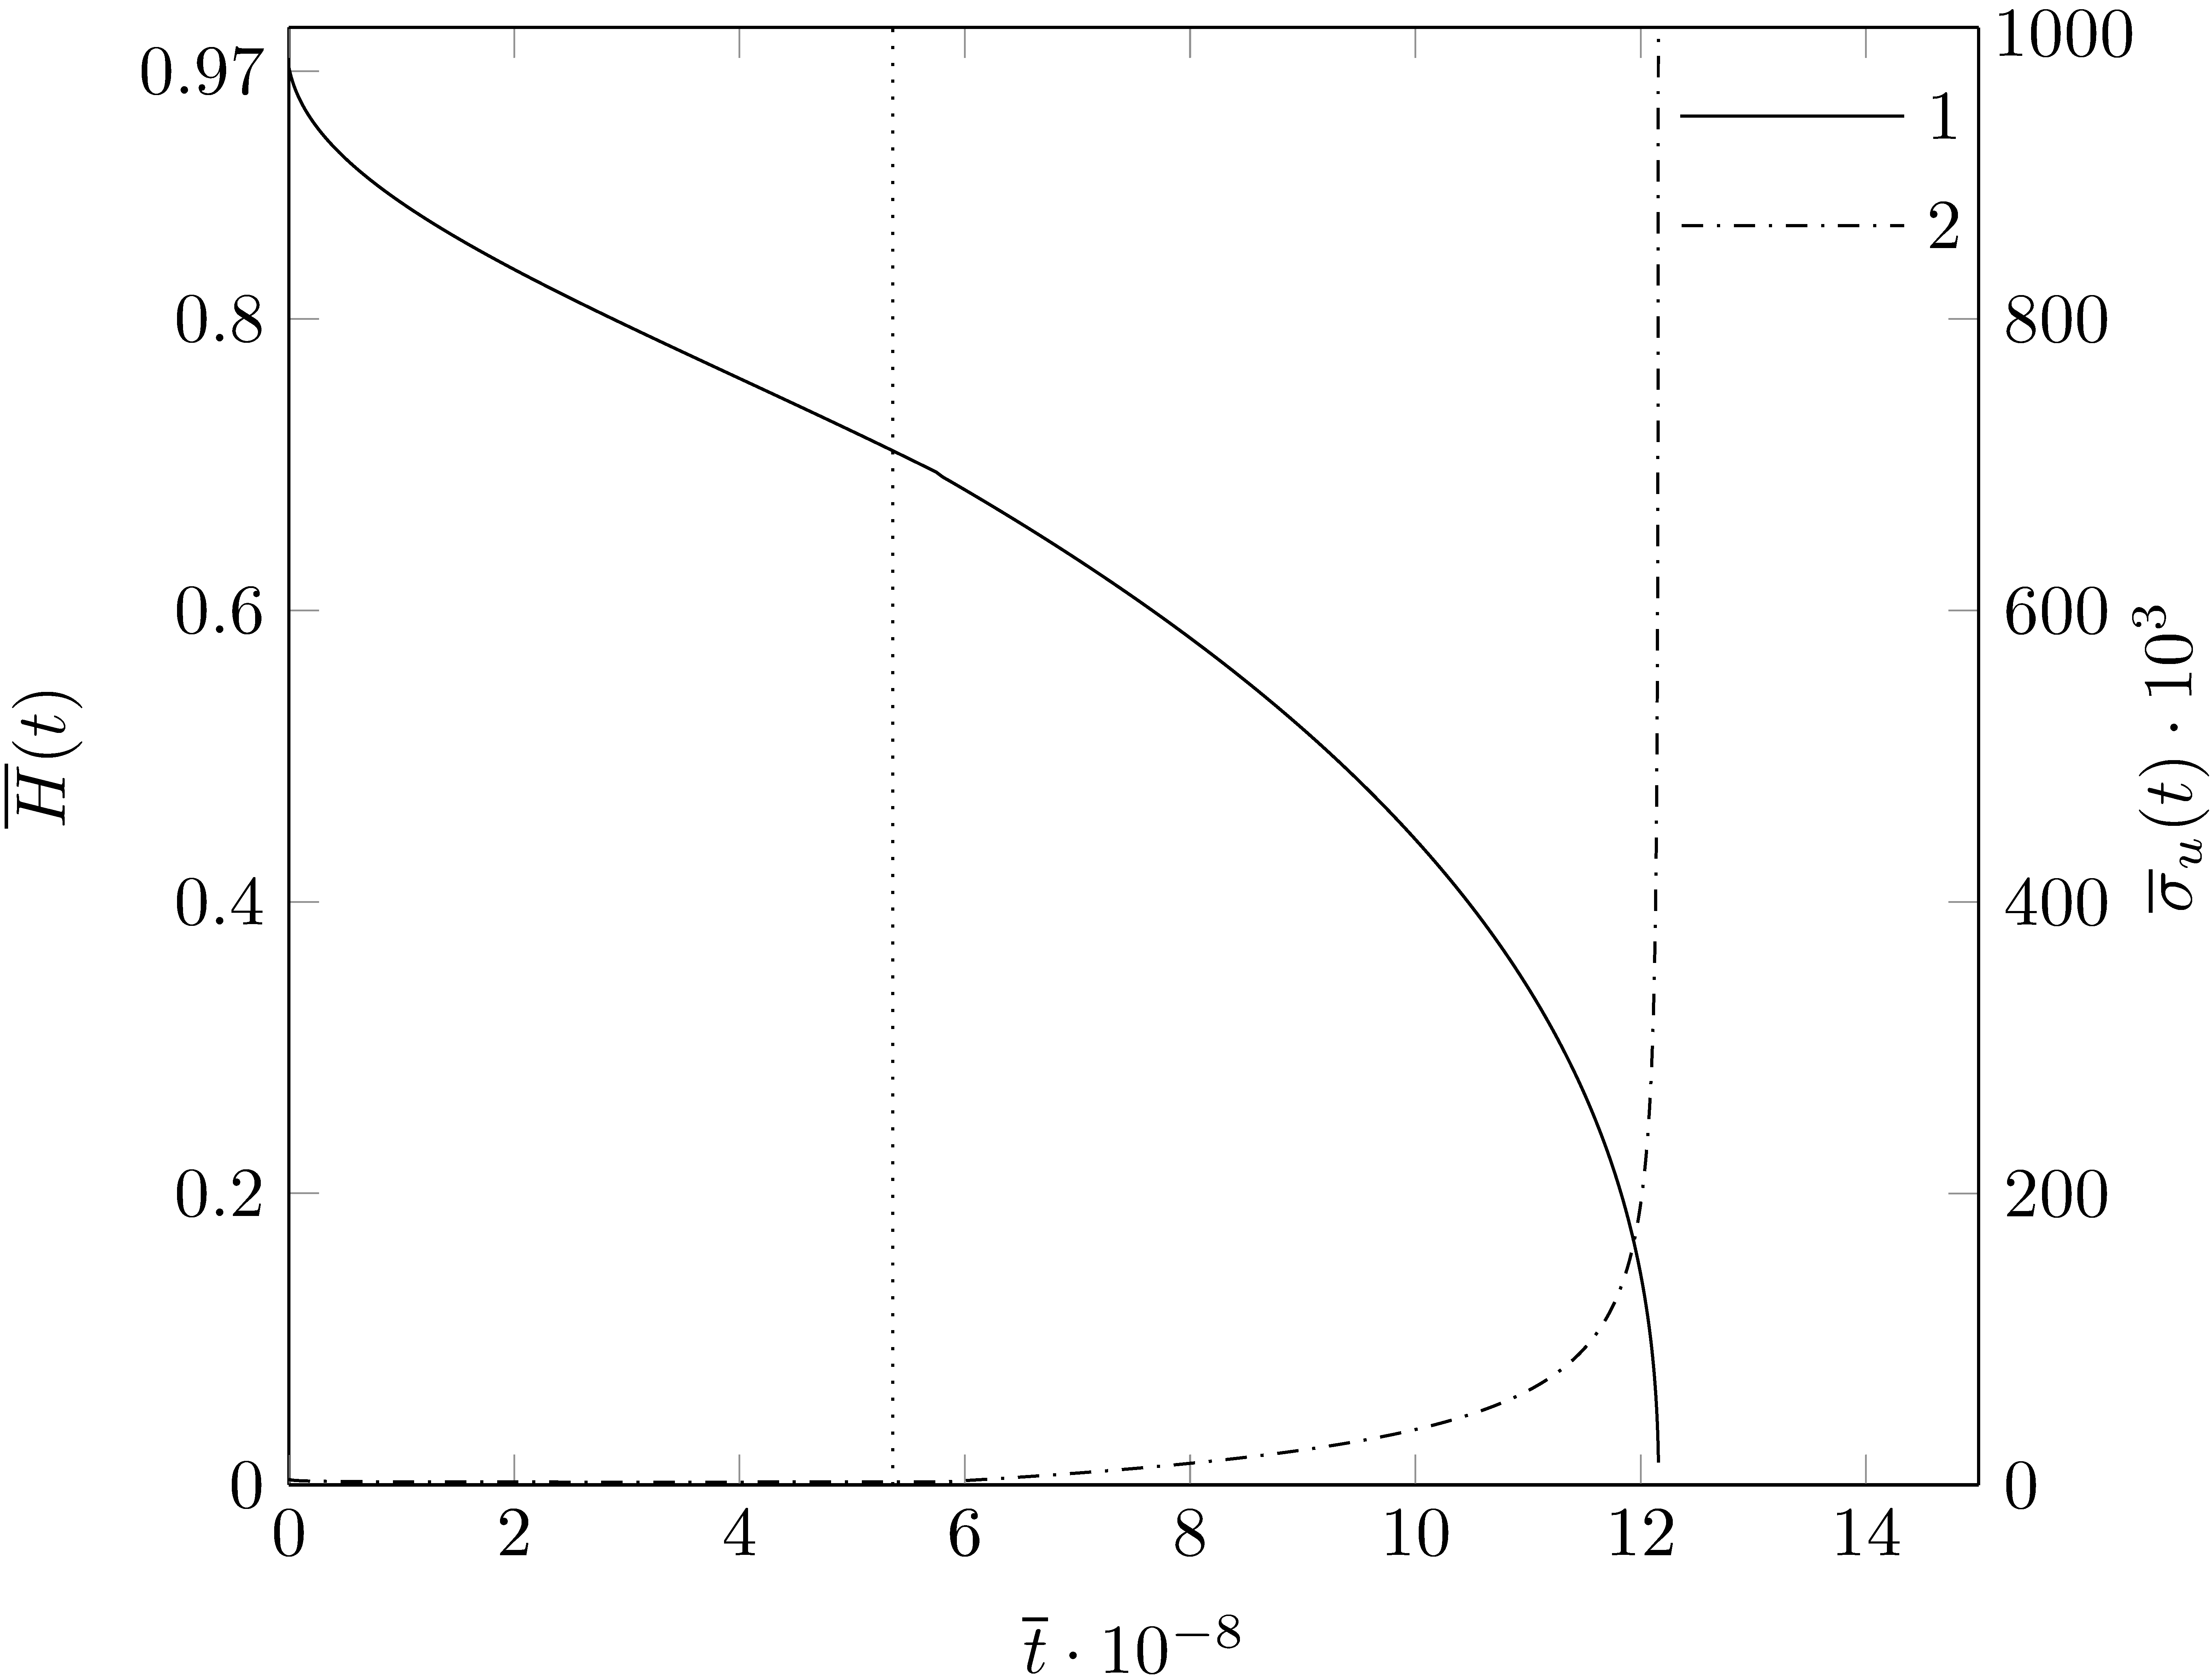
\includegraphics[width=0.9\linewidth]{images/quad_sticking.png}}
				\caption{} 
				\label{quad_sticking}
		\end{figure}

		
		Расчет для мембраны внутри матрицы с вертикальными стенками и плоским днищем проводился для матриц с различной высотой:
		$b = a$ (рис.\ref{vert_sliging_ba}), $b = 4.5a$ (рис.\ref{vert_sliging_4ba}),$b=7a$ (рис.\ref{vert_sliging_7ba}), $b=10a$ (рис.\ref{vert_sliging_10ba}). Из рисунков видно, что при увеличении высоты мембраны увеличивается максимально достижимая интенсивность напряжения, которая при достижении значения $\sigma_b$ приведет к разрушению мембраны. Но само разрушение в данной работе не рассматривалось.
Приведем результаты вычислений в таблице \ref{vert_table}
\begin{center}

\renewcommand{\arraystretch}{2}
\begin{tabular}{|c|c|c|}
\hline
$b/a$    & $\overline{t_2}$/$\overline{H_2}$ & $\overline{t_3}$/$\overline{H_3}$ \\
\hline\hline
1    & $7.14\cdot10^8$/0.636  & $7.14\cdot10^8$/0.636\\ \hline
4.5  & $7.14\cdot10^8$/0.636  & $13.67\cdot10^8$/0.186\\ \hline
7    & $7.14\cdot10^8$/0.636  & $13.96\cdot10^8$/0.125\\ \hline
10   & $7.14\cdot10^8$/0.636  & $13.98\cdot10^8$/0.089\\ \hline

\end{tabular}
\label{vert_table}
\end{center}
				 
		\begin{figure}[h!]	
				\def\svgwidth{\columnwidth}
				\center{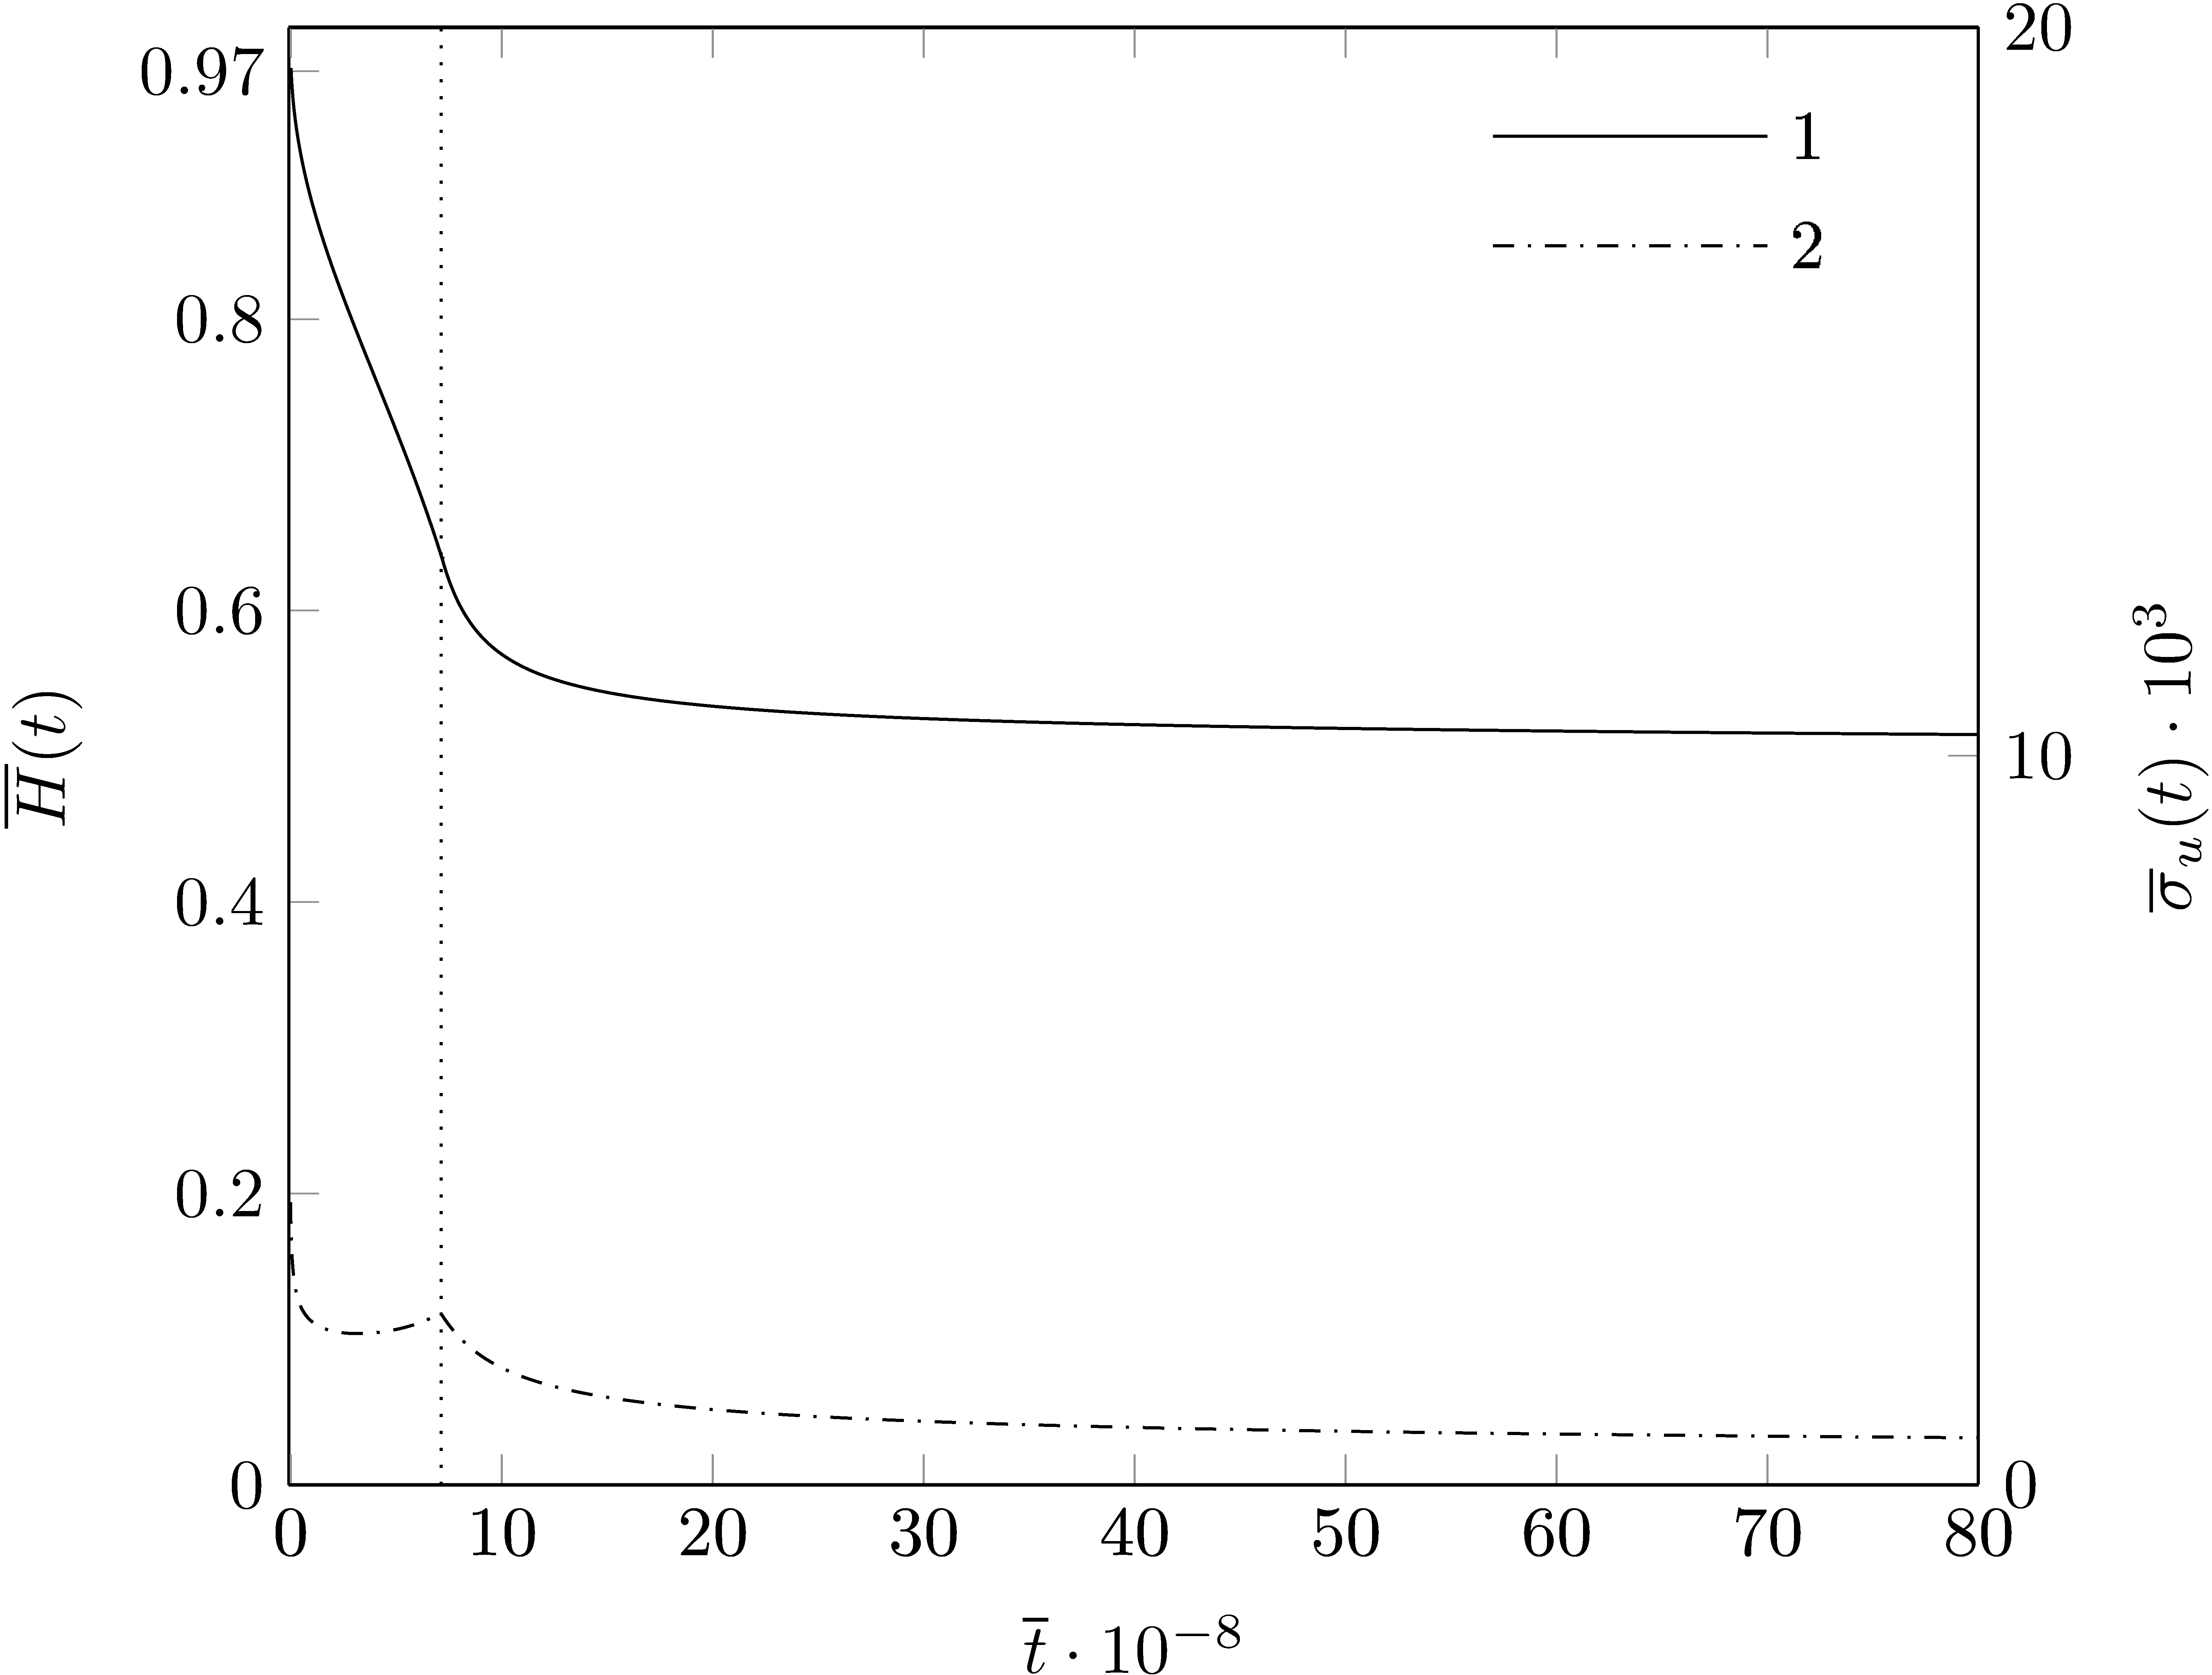
\includegraphics[width=0.9\linewidth]{images/ab.png}}
				\caption{b=a} 
				\label{vert_sliging_ba}
		\end{figure}

		\begin{figure}[h!]	
				\def\svgwidth{\columnwidth}
				\center{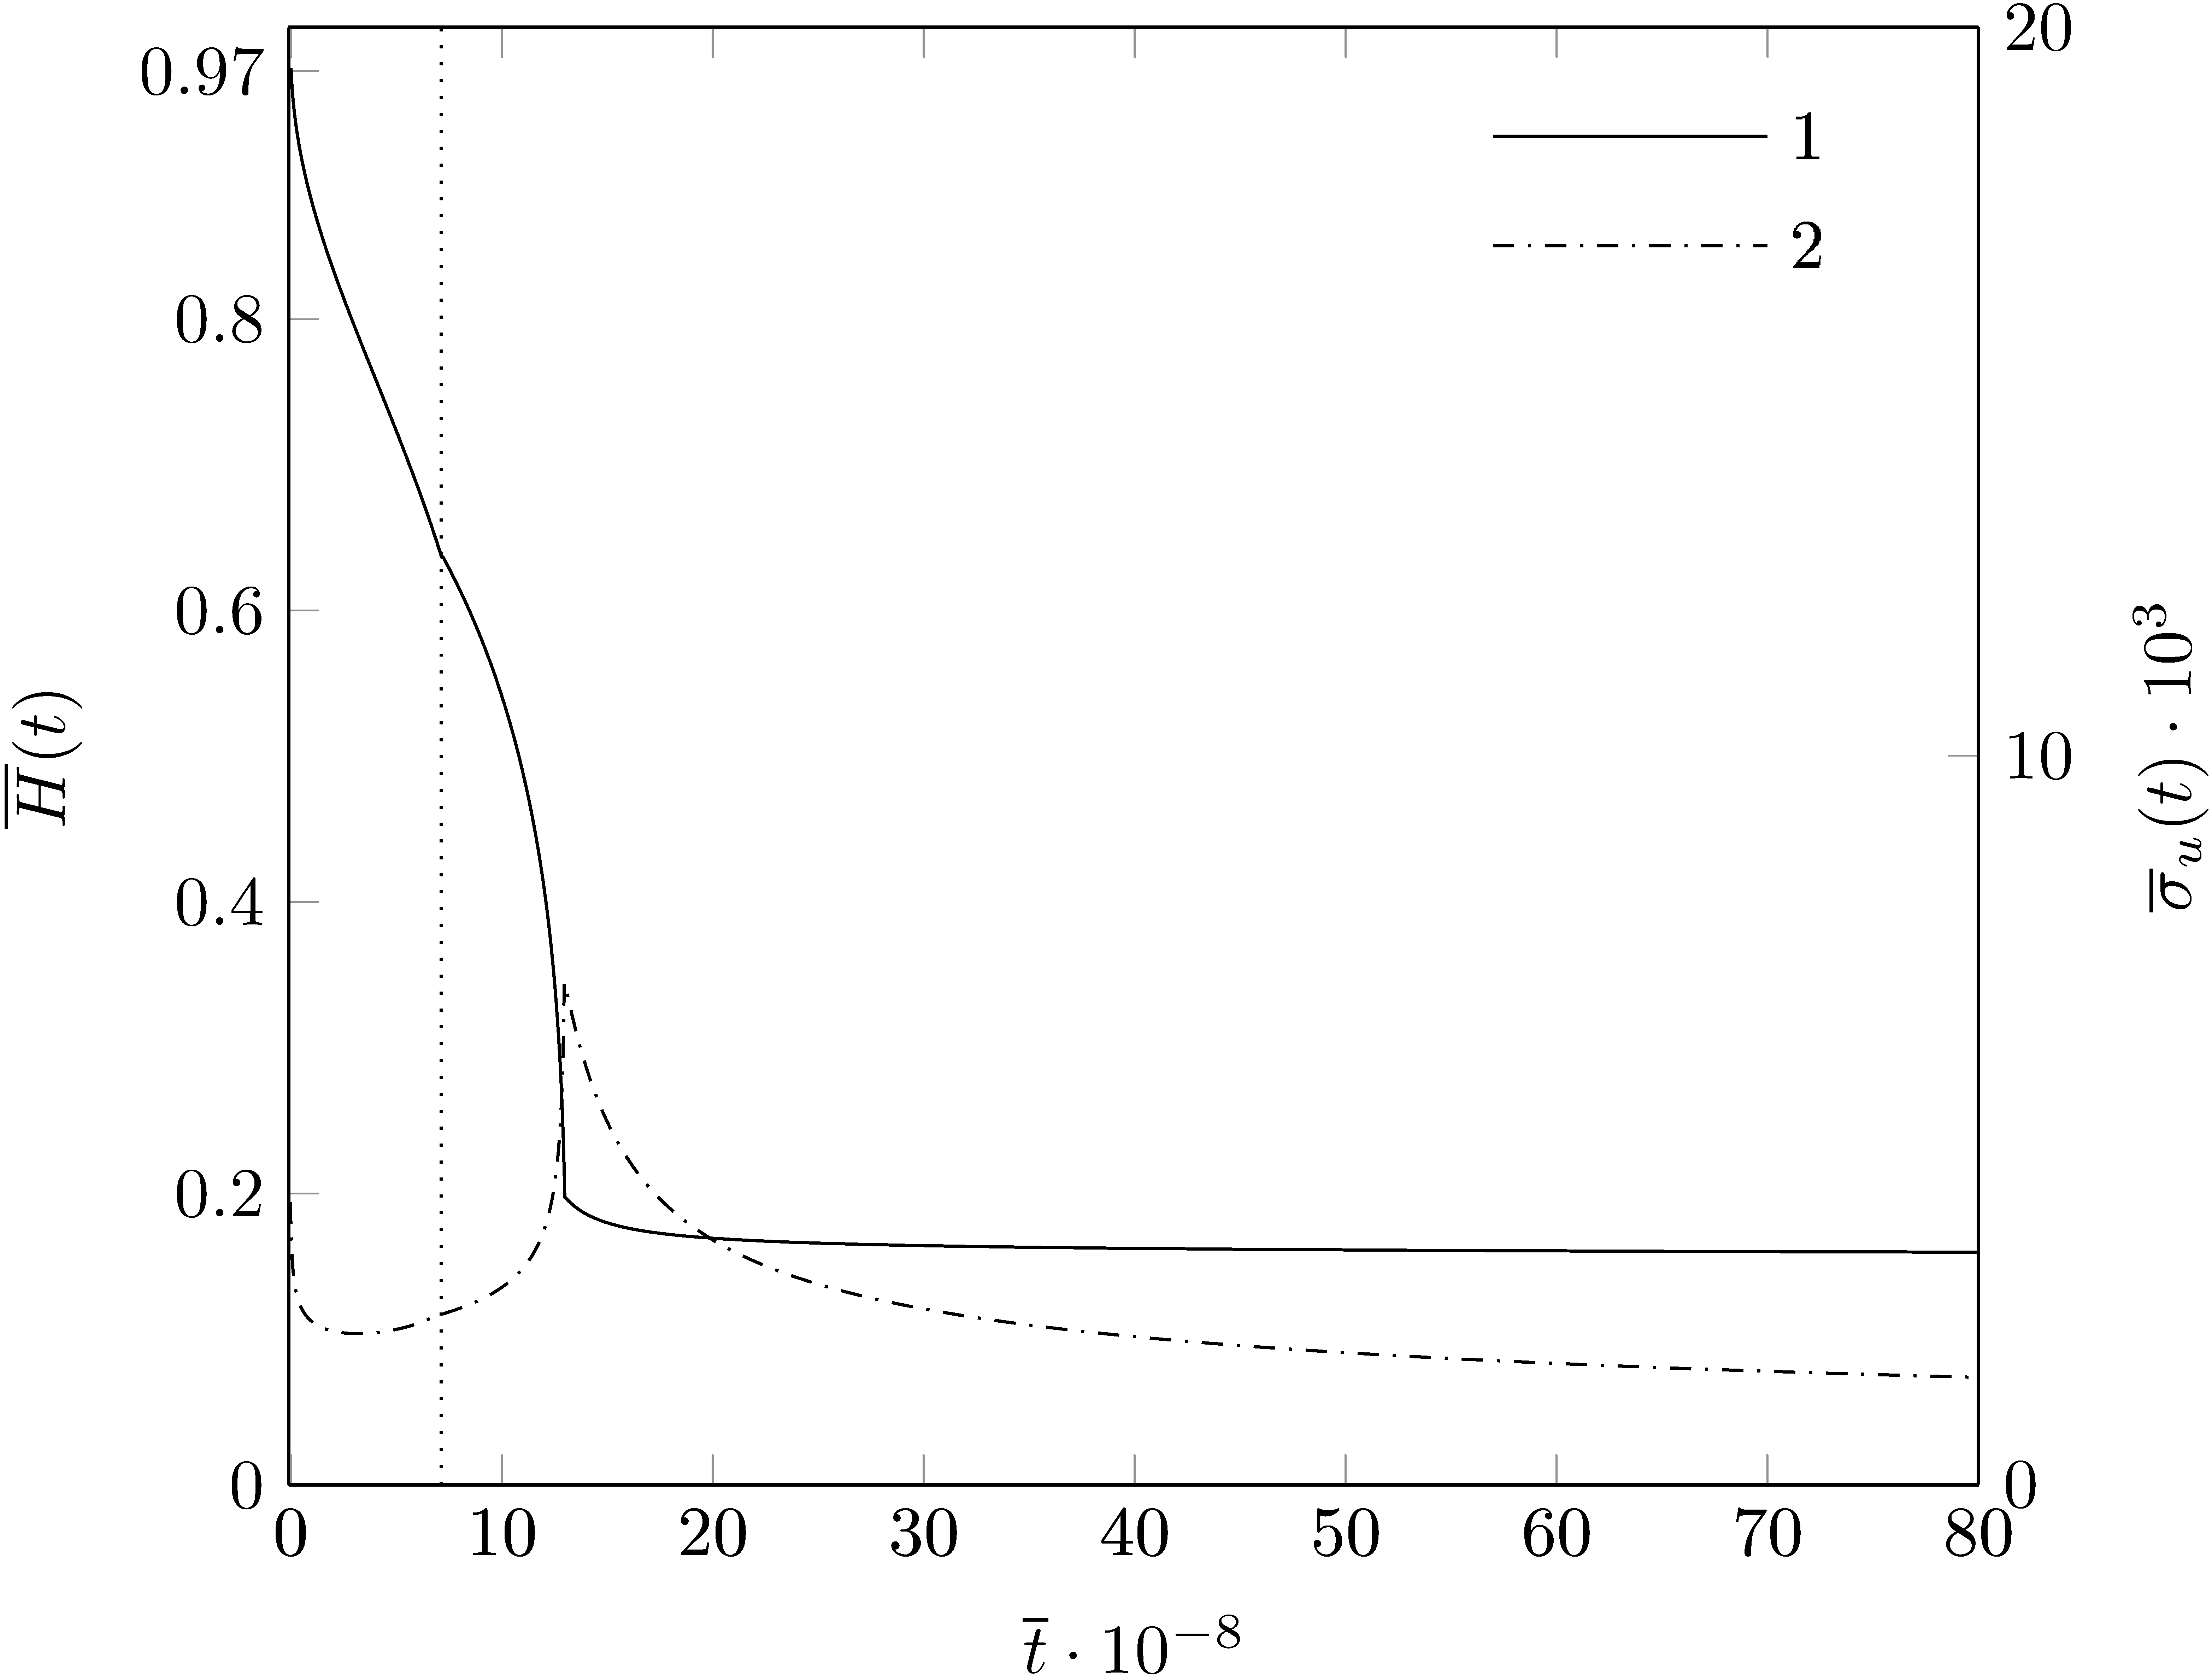
\includegraphics[width=0.9\linewidth]{images/ab4.png}}
				\caption{b=a} 
				\label{vert_sliging_4ba}
		\end{figure}
				\begin{figure}[h!]	
				\def\svgwidth{\columnwidth}
				\center{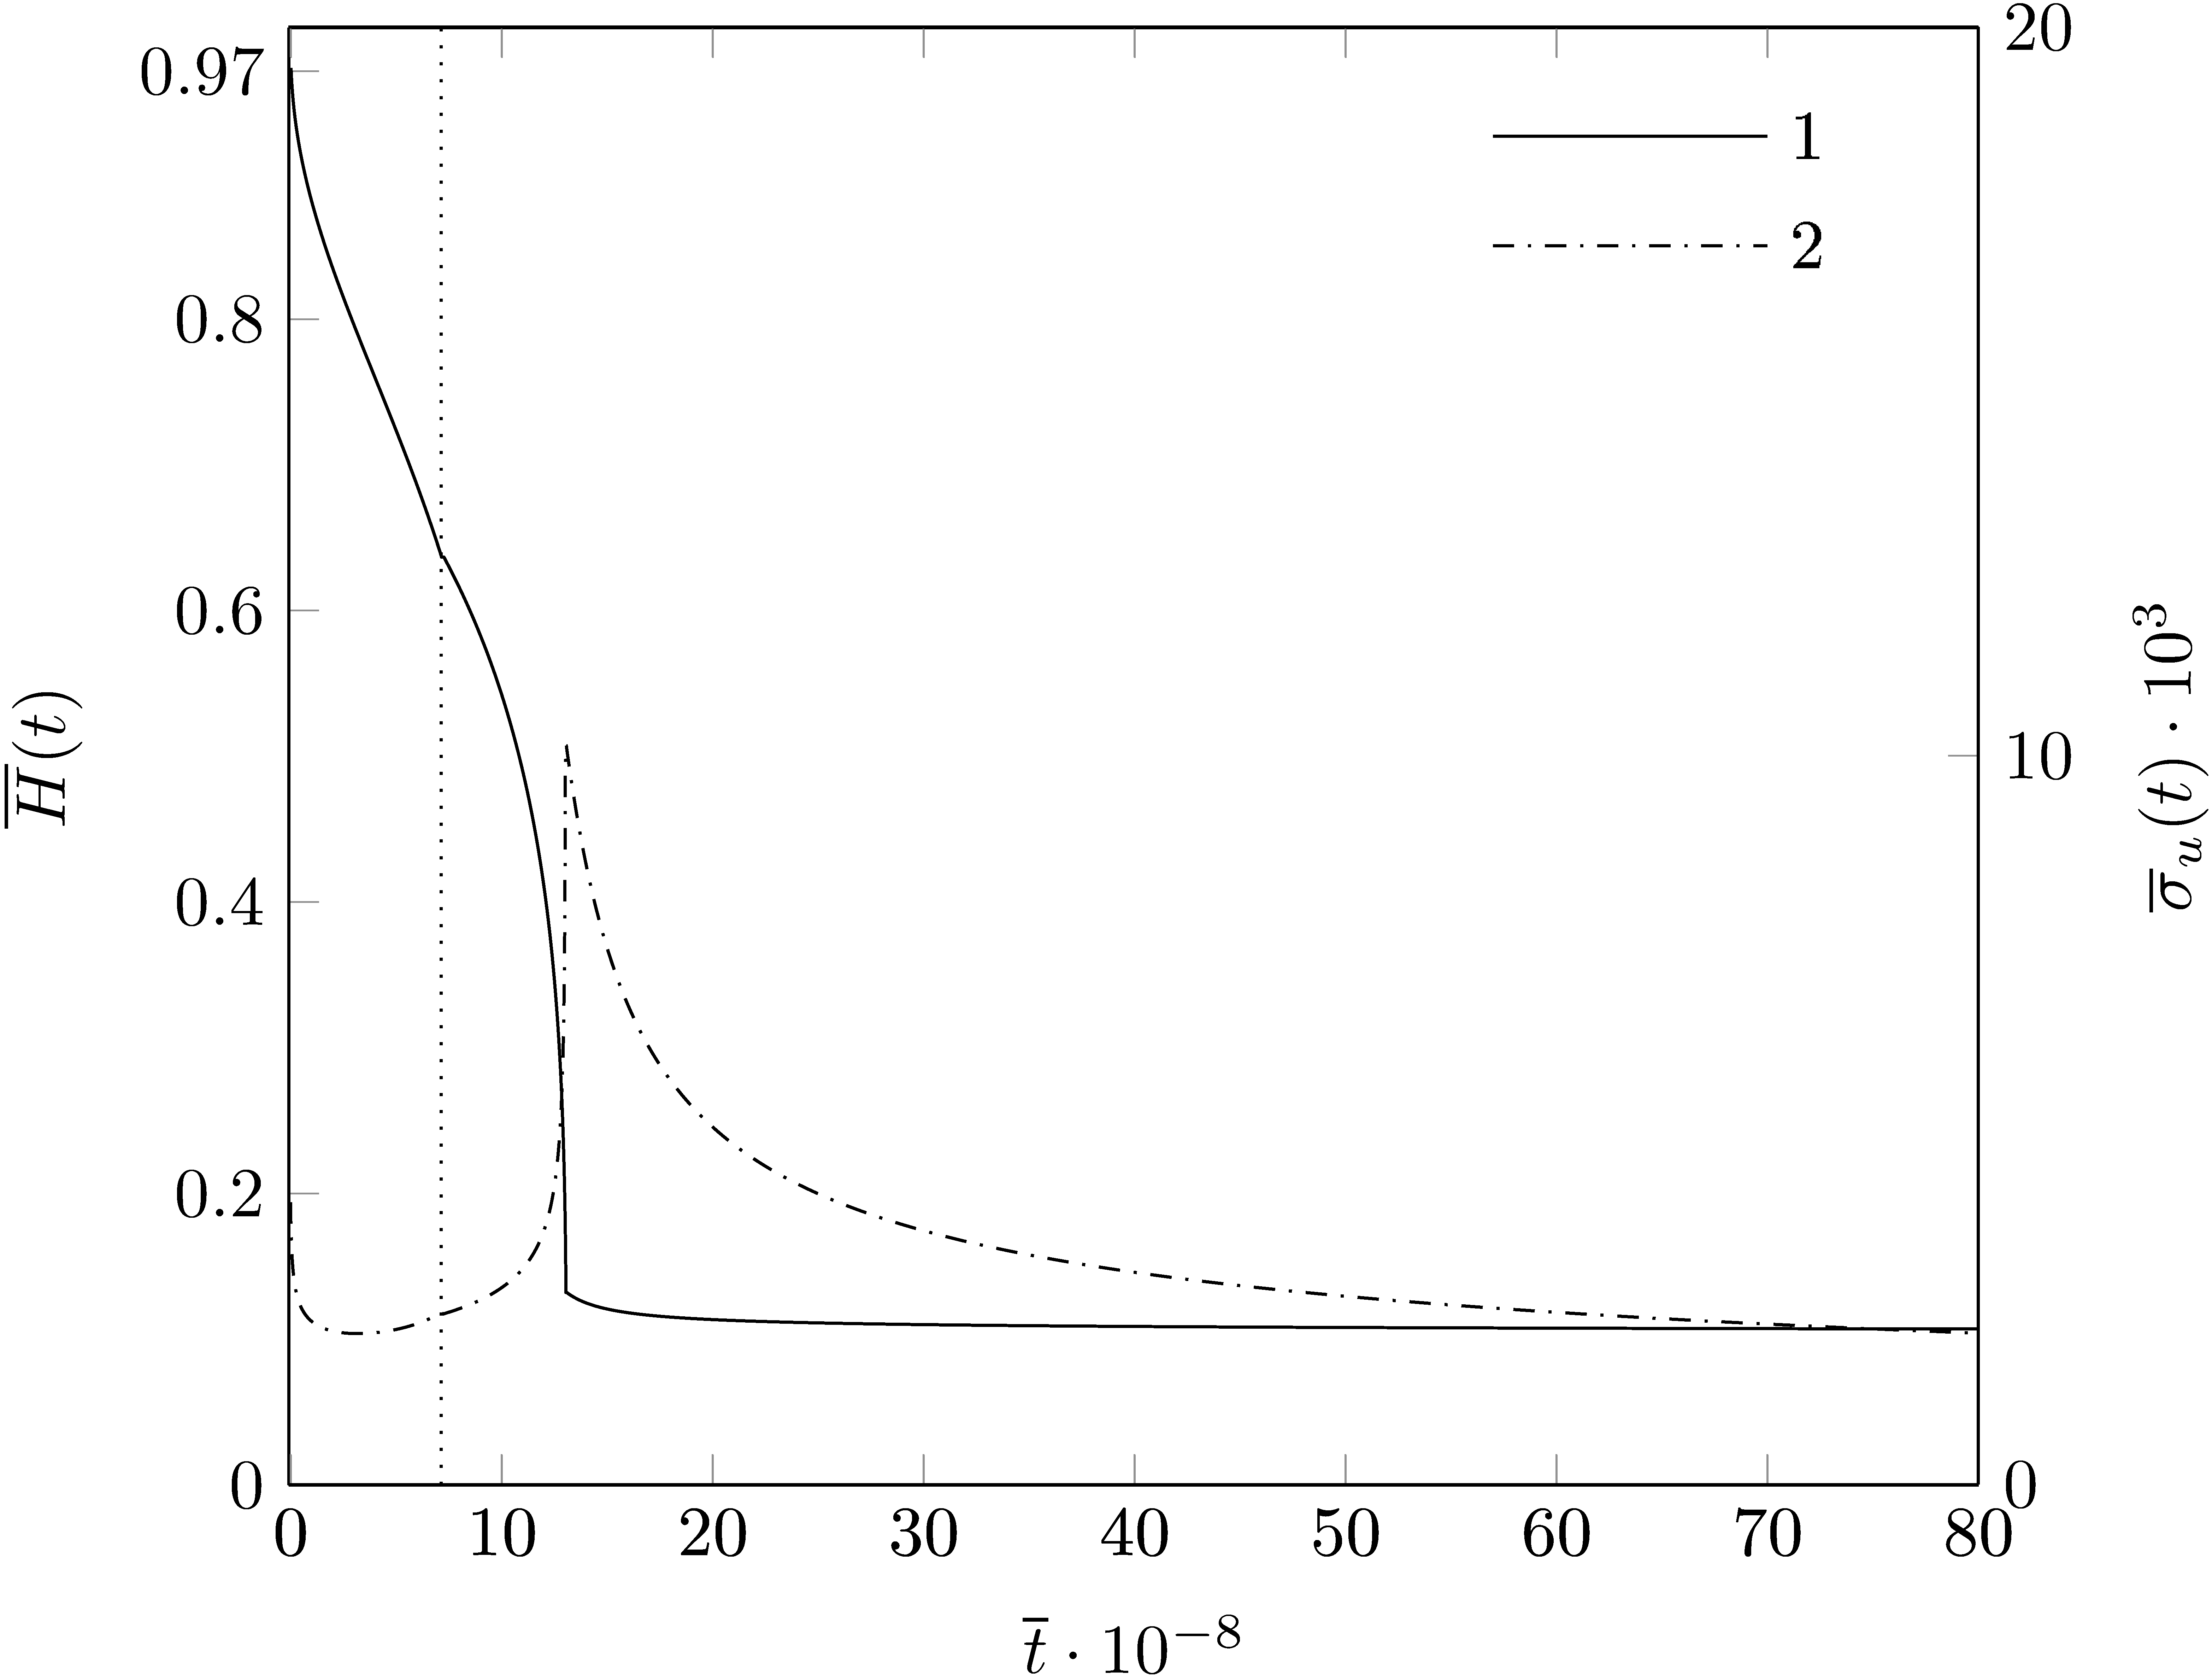
\includegraphics[width=0.9\linewidth]{images/ab7.png}}
				\caption{b=a} 
				\label{vert_sliging_7ba}
		\end{figure}
				\begin{figure}[h!]	
				\def\svgwidth{\columnwidth}
				\center{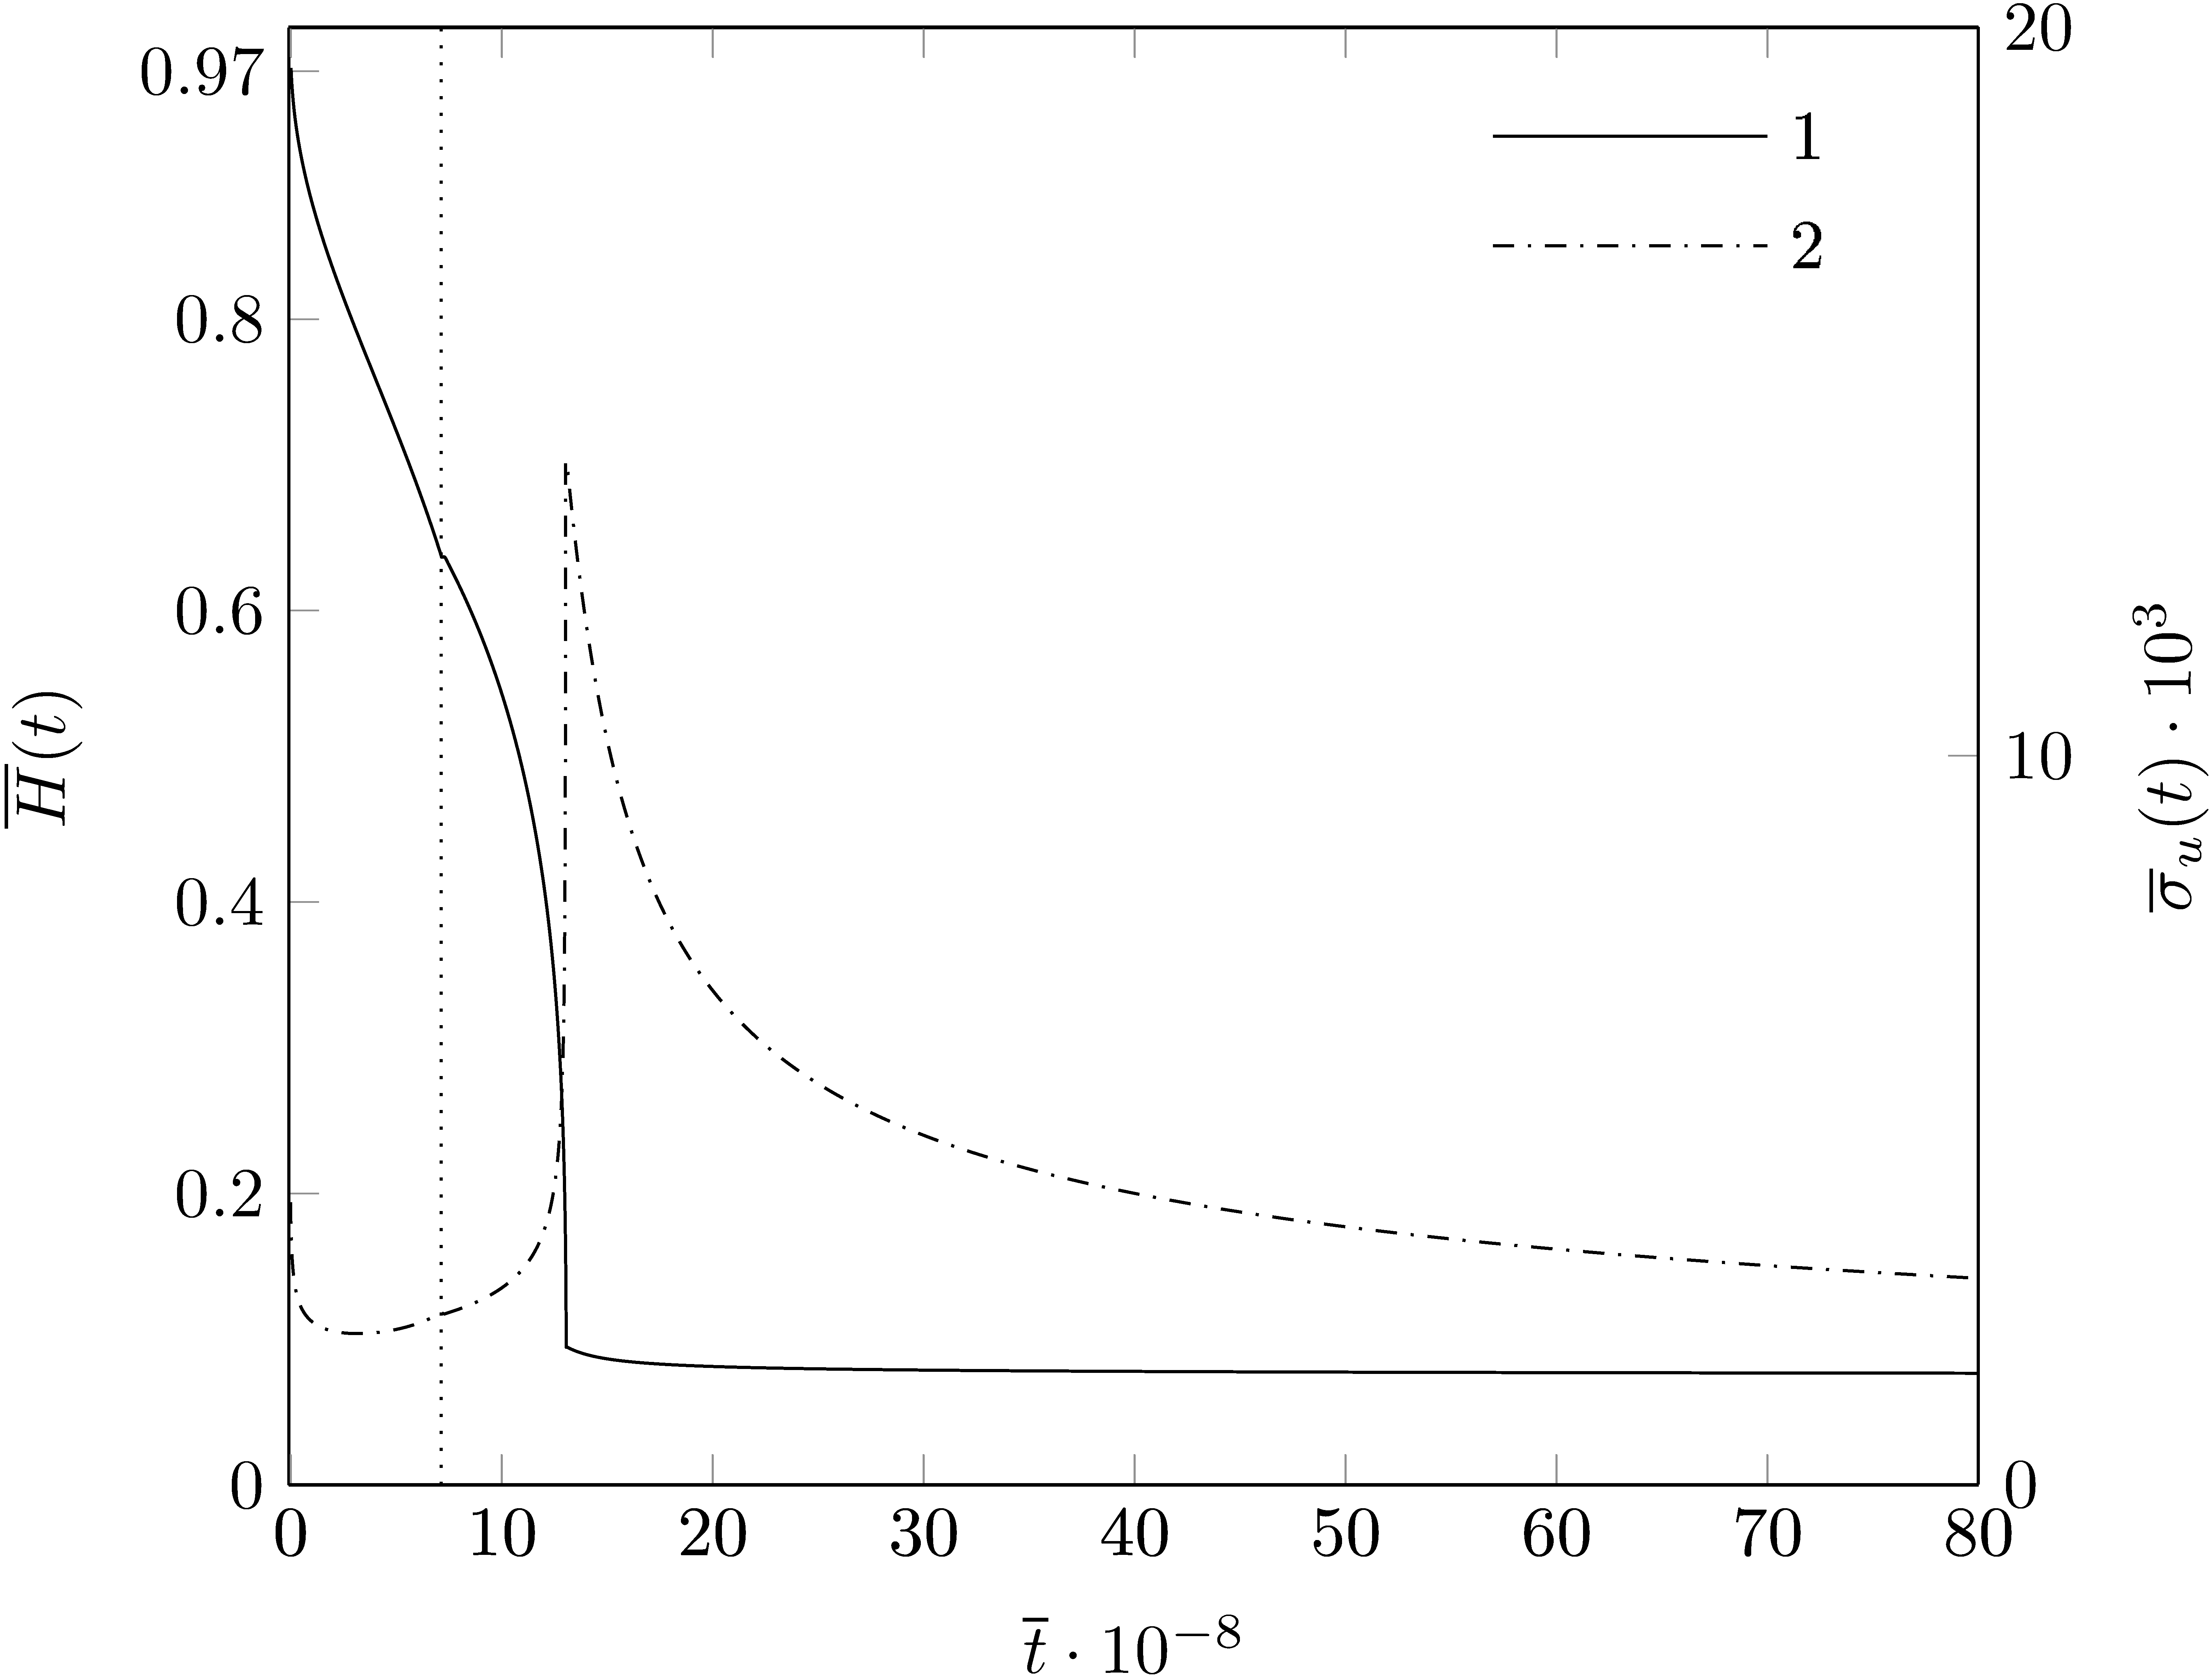
\includegraphics[width=0.9\linewidth]{images/ab10.png}}
				\caption{b=a} 
				\label{vert_sliging_10ba}
		\end{figure}

Для другого граничного условия так же были проведен численный расчет и были получены следующие результаты:
Для
		
\clearpage
\section{Анимирование}
